%%%%%%%%%%%%%%%%%%%%%%%%%%%%%%%%%%%%%%%%%%%%%%%%%%%%%%%%%%%%%%%%%%%%%%%%%%%%%%%%
%%    Rnw PROGRAM: screenr_Tutorial.Rnw
%%
%%    R PACKAGE: screenr
%%
%%    Usage: knit("screenr_Tutorial.Rnw")
%%
%%    DESCRIPTION: A LaTeX pdf version of the tutorial
%%%%%%%%%%%%%%%%%%%%%%%%%%%%%%%%%%%%%%%%%%%%%%%%%%%%%%%%%%%%%%%%%%%%%%%%%%%%%%%%


%%%%%%%%%%%%%%%%%%%%%%%%%%%%%%%%%%%%%%%%%%%%%%%%%%%%%%%%%%%%%%%%%%%%%%%%%%%%%%%%
%% LaTeX Preamble
%%%%%%%%%%%%%%%%%%%%%%%%%%%%%%%%%%%%%%%%%%%%%%%%%%%%%%%%%%%%%%%%%%%%%%%%%%%%%%%%
\documentclass[11pt]{report}
\usepackage[numbers]{natbib}
%%\usepackage{amsmath,amssymb,amsfonts}
\usepackage{textcomp}
\usepackage[font={footnotesize},labelfont={bf},labelsep=period]{caption}
\usepackage[utf8x]{inputenc}
\usepackage{hyperref}
\usepackage{cite}
\usepackage{float}
%%\usepackage{booktabs}
\usepackage{graphicx}
\usepackage{fancyvrb}
\usepackage{afterpage}
%%  Increase the height of printing in pages
\addtolength{\topmargin}{-.875in}
\addtolength{\textheight}{1.75in}
%%  Increase the text width
\addtolength{\hoffset}{-0.5in}
\addtolength{\textwidth}{1in}
%%  Alter some LaTeX defaults for better treatment of figures:
%%  See p.105 of "TeX Unbound" for suggested values.
%%  See pp. 199-200 of Lamport's "LaTeX" book for details.
%%      General parameters, for ALL pages:
\renewcommand{\topfraction}{0.9}	      % max fraction of top floats
\renewcommand{\bottomfraction}{0.8}	      % max fraction of bottom floats
%%  Parameters for TEXT pages (not float pages):
\setcounter{topnumber}{2}
\setcounter{bottomnumber}{2}
\setcounter{totalnumber}{4}               % 2 may work better
\setcounter{dbltopnumber}{2}              % for 2-column pages
\renewcommand{\dbltopfraction}{0.9}	      % fit big float above 2-col. text
\renewcommand{\textfraction}{0.07}	      % allow minimal text w. figs
%%  Parameters for FLOAT pages (not text pages):
\renewcommand{\floatpagefraction}{0.7}	  % require fuller float pages
%%  N.B.: floatpagefraction MUST be less than topfraction !!
\renewcommand{\dblfloatpagefraction}{0.7} % require fuller float pages
%%  Caption customizations
\captionsetup[figure]{width=0.9\textwidth}
%%  Graphics width
\setkeys{Gin}{width=0.99\textwidth, clip=TRUE, keepaspectratio=TRUE}
\renewcommand{\bibname}{References}
\renewcommand{\figurename}{Fig}

%%  Customizations:
\usepackage{Sweave}

\DefineVerbatimEnvironment{Sinput}{Verbatim}{fontsize=\footnotesize,fontshape=n,xleftmargin=2em}
\DefineVerbatimEnvironment{Soutput}{Verbatim}{fontsize=\footnotesize,fontshape=n,xleftmargin=2em}
\DefineVerbatimEnvironment{Scode}{Verbatim}{fontsize=\footnotesize,fontshape=n,xleftmargin=2em}
\fvset{listparameters={\setlength{\topsep}{0pt}}}
\renewenvironment{Schunk}{\vspace{\topsep}}{\vspace{\topsep}}

%%  Title and author(s):
\title{\textsf{\textbf{screenr Tutorial}}}
%%\author{Steve Gutreuter \\ \href{mailto:sgutreuter@gmail.com}{sgutreuter@gmail.com}}

%%%%%%%%%%%%%%%%%%%%%%%%%%%%%%%%%%%%%%%%%%%%%%%%%%%%%%%%%%%%%%%%%%%%%%%%%%%%%%%%
%% BEGIN DOCUMENT

\begin{document}
\begin{center}
  \Huge{\textbf{screenr Tutorial}} \\
  \vspace{1em}
%%  \Large{Steve Gutreuter} \\
%%  \normalsize{\href{mailto:sgutreuter@gmail.com}{sgutreuter@gmail.com}}
\end{center}

\section*{Introduction}

% The \textsf{screenr} package eases the development and validation of
% pre-testing screening tools of the sort reviewed by Clemens et
% al\citep{Clemens+al2020}, but is applicable to any test-screening
% problem. Universal testing for a condition can be impractical if the
% test procedure is relatively expensive and the condition is rare.
% Alternatively, testing only those subjects having a sufficiently large
% probability of testing positive may be viable if a screening procedure
% can be developed which has an acceptable
% \href{https://en.wikipedia.org/wiki/Sensitivity_and_specificity}{sensitivity}.
% That may be possible if easily measured/recorded risk factors for test
% positivity can be identified.

% This vignette demonstrates the development and validation of such a
% screening tool using lasso-like \emph{L}1
% \href{https://towardsdatascience.com/regularization-in-machine-learning-76441ddcf99a}{regularization}\citep{Hastie+al2009}
% of logistic models, as implemented in the glmpath
% package\citep{Park+Hastie2007}, and also model fitting using
% maximum-likelihood estimation.  Regularization enables robust model
% selection, but the parameter estimates are biased toward zero.
% Therefore one might choose to re-fit the model selected by
% regularization using maximum-likelihood estimation.  Model performance
% is evaluated using receiver-operating characteristics (ROC)
% \citep{Fawcett2006,Streiner+Cairney2007,Robin+al2011}.


\section*{An (Artificial) Example}

\href{https://www.britannica.com/topic/unicorn}{Unicorns} suffer an
epidemic of infection by the Unicorn Immunodeficiency Virus (UIV).
There is currently no cure for UIV infection, but highly effective
antiretrovial therapy has the potential to block forward
transmission and to avert death from opportunistic infections
associated with UIV infection.  Therefore it is critical
that UIV infection is detected, and that infected unicorns are
enrolled in treatment.  However, UIV infection is sufficiently rare
that universal testing of unicorns at health-care entry points is
impractical.  The challenge then is to identify
unicorns who should be prioritized for testing.

A sample of 6000 properly consented adult unicorns
were enrolled in a study aimed at evidence-based targeting of testing
for UIV infection.  The subjects were administered a questionnaire
identifying the presence or absence of putative risk factors for UIV
infection.  The prevalence of UIV is low, and therefore universal
testing was deemed impractical. Because UIV is
transmissible and fatal if left untreated, it is important that the
screening tool have an acceptably high sensitivity.  The
\textsf{screenr} package enables development and validation of such
screening tools.

The screening questionnaire included seven questions which were
selected based on published information on infection risk. The data
consists of the responses to the screening questions \textsf{Q1, ..., Q7}
(coded as 1 for an affirmative response and 0 for a negative
response), and the testing outcome (\textsf{testresult}), again coded 0 and 1
for negative and positive results, respectively.

\textbf{NOTE:} It is critically important that all of the putative risk
factors have a \emph{positive} association with the outcome.  That is, the
questionnaire must be designed so that affirmative (yes) responses are
hypothesized to indicate an \emph{increased} risk of UIV infection.

The data from the unicorn study look like:

\begin{Schunk}
\begin{Sinput}
R> ## The first six lines of the unicorn screening data:
R> head(unicorns)
\end{Sinput}
\begin{Soutput}
  ID Q1 Q2 Q3 Q4 Q5 Q6 Q7 testresult
1  1  0  0  0  0  0  0  1          0
2  2  0  0  0  0  0  0  0          0
3  3  0  0  0  0  0  0  0          0
4  4  1  0  0  0  0  0  1          0
5  5  1  0  0  1  1  0  1          0
6  6  0  0  0  0  0  0  0          0
\end{Soutput}
\end{Schunk}

The prevalence of UIV in the sample of unicorns is
0.016. Under universal testing
at health-care entry points, discovery of a single
infection would require, on average, testing
62 unicorns.

\section*{Screening Tool Development}

This demonstration of screening-tool development and
validation consists of five steps:
\begin{enumerate}
\item Model selection
\item Refitting the final model
\item Selection of a screening threshold
\item External validation on entirely new data
\item Implementation
\end{enumerate}

In practice, unfortunately, the fourth step is sometimes omitted due to
resource limitations.

\subsection*{Model selection}

The first step is the selection of a parsimonious logistic screening
model.  A method known as \emph{L}1 regularization has desirable
properties for that task\citep{Hastie+al2009,Park+Hastie2007}.  The
function \textsf{lasso\_screenr()} provides easy, integrated access to
the \emph{L}1 regularization algorithm of Park and
Hastie\citep{Park+Hastie2007}, as implemented in the \textsf{glmpath}
\textsf{R} package, using a convenient formula interface:
\begin{Schunk}
\begin{Sinput}
R> uniobj1 <- lasso_screenr(testresult ~ Q1 + Q2 + Q3 + Q4 + Q5 + Q6 + Q7,
+                          data = unicorns, Nfolds = 10, seed = 123)
\end{Sinput}
\end{Schunk}

The formula \verb|testresult ~ Q1 + Q2 + Q3 + Q4 + Q5 + Q6 + Q7| is an
expression of the statement ``predict \verb|testresult| from the seven
covariates \verb|Q1, ..., Q7|''. The argument \verb|Nfolds = 10|
specifies the desired number of partitions (folds) to be used for
cross validation (discussed under \textbf{Selection of a screening
threshold}, below).  The optional \verb|seed| argument specifies the starting value
for the random-number generator used for cross-validation data-splitting. Here
it is set to a fixed value to insure reproducibility. By default, the
seed is set by the system clock, and therefore results will vary from
run to run. Set the seed only if reproducible results are needed.

The fitting algorithm computes logit-scale coefficients along the
entire regularization path, and has the effect of selecting covariates
based on penalization by the
\emph{L}1-\href{https://towardsdatascience.com/norms-penalties-and-multitask-learning-2f1db5f97c1f}{norm}
of their coefficients, similar to the ordinary
lasso\citep{Hastie+al2009}.  Unlike the ordinary lasso, the
algorithm can also impose a very small penalty on the \emph{L}2-norm,
which eliminates adverse effects of any strong correlations among the
predictors and provides useful estimates even if the response variable
is separable by the predictors (albeit unlikely in test-screening
applications).

\textbf{IMPORTANT:} The object returned by \textsf{lasso\_screenr} (or any of the other
\textsf{"\_screenr"} functions) contains information critical to validation and
implementation of test screening. Therefore \textbf{the object should be saved
for future use}, for example:
\begin{Schunk}
\begin{Sinput}
R> saveRDS(uniobj1, file = "uniobj1.rds" )
\end{Sinput}
\end{Schunk}

The resulting \textsf{lasso\_screenr}-class object (\textsf{uniobj1})
includes the results from regularization, and performance measures from
the fits to all of the data using \emph{k}-fold cross validation.
\textsf{uniobj1}, contains all of the information need to develop and
(internally) validate a screening tool for diagnostic tests. The
\textsf{screenr} package provides the following methods for
\textsf{lasso\_screenr}-class objects:
\begin{Schunk}
\begin{Sinput}
R> methods(class = "lasso_screenr")
\end{Sinput}
\begin{Soutput}
[1] coef     get_what ntpp     plot     predict  print    summary
see '?methods' for accessing help and source code
\end{Soutput}
\end{Schunk}
The methods should make it mostly unnecessary to access components of
\textsf{lasso\_screenr}-class objects directly using \textsf{R} code similar to
\verb|object$component|.

For example, the \verb|summary| method provides basic information about the results
of regularization:
\begin{Schunk}
\begin{Sinput}
R> summary(uniobj1)
\end{Sinput}
\begin{Soutput}
  Step Df Deviance     AIC      BIC     pAUC  pAUClcl  pAUCucl
1    1  1  992.635 994.635 1001.335 0.500000 0.500000 0.500000
2    2  2  909.422 913.422  926.822 0.641458 0.585151 0.727844
3    3  3  883.554 889.554  909.653 0.805897 0.754572 0.848602
4    5  4  738.400 746.400  773.198 0.810232 0.755625 0.859306
5    7  5  717.198 727.198  760.696 0.830873 0.778376 0.876674
6    8  6  687.054 699.054  739.251 0.838530 0.791346 0.881856
7   11  7  680.954 694.954  741.851 0.840741 0.792496 0.883218
8   12  8  680.952 696.952  750.549 0.848432 0.803474 0.889282
\end{Soutput}
\end{Schunk}
Regularization yielded eight models. Two solutions along the
regularization path which yield the smallest
\href{https://docs.displayr.com/wiki/Information_Criteria}{AIC and
BIC} values, denoted \verb|"minAIC"| and \verb|"minBIC"|,
respectively, are given special status.  Those are likely the most
useful solutions in nearly all settings.  The default for pAUC is the
area under the ROC curve for which sensitivity is at least 0.8, but
see the results of \verb|help(lasso_screenr)| for other
options. However all solutions are accessible from
\textsf{lasso\_screenr}-class objects.

The logit-scale coefficients for the two special models
are obtained using:
\begin{Schunk}
\begin{Sinput}
R> coef(uniobj1)
\end{Sinput}
\begin{Soutput}
          AIC.best.model BIC.best.model
Intercept      -7.568603   -6.833257953
Q1              2.767832    2.468497841
Q2              1.560257    1.100266591
Q3              2.891689    2.575660525
Q4              0.000000    0.000000000
Q5              1.822216    1.578669298
Q6              0.363779    0.000656197
Q7              0.843276    0.581431699
\end{Soutput}
\end{Schunk}
Note that the coefficients for Q4 have been shrunk to zero in both the
AIC- and BIC-best models. In effect, Q4 has been eliminated from both
of those models because it was not an important predictor of test
positivity. One can also obtain the adjusted odds ratios and/or omit the
intercept.  For example, the adjusted odds ratios for the seven
predictors can be obtained using:
\begin{Schunk}
\begin{Sinput}
R> coef(uniobj1, or = TRUE, intercept = FALSE)
\end{Sinput}
\begin{Soutput}
   AIC.best.model BIC.best.model
Q1       15.92408       11.80470
Q2        4.76004        3.00497
Q3       18.02373       13.13999
Q4        1.00000        1.00000
Q5        6.18555        4.84850
Q6        1.43876        1.00066
Q7        2.32397        1.78860
\end{Soutput}
\end{Schunk}
The adjusted odds ratios for Q4 are 1.0, again indicating that Q4 was
not predictive of the test result.  One can also examine the
coefficients everywhere the active set changed along the
regularization path for either of the special fits by extracting and
plotting the regularization path object:
\begin{Schunk}
\begin{Sinput}
R> pathobj <- get_what(from = uniobj1, what = "glmpathObj", model = "minAIC")
\end{Sinput}
\end{Schunk}
\begin{figure}[!h]
  \begin{center}
\begin{Schunk}
\begin{Sinput}
R> plot(pathobj, xvar = "lambda", main = "")
\end{Sinput}
\end{Schunk}
\includegraphics{FIXME-011}
\caption{Plot of model coefficient values along the regularization
  path.}
\label{fig:f1}
\end{center}
\end{figure}
Figure \ref{fig:f1} is produced using the \textsf{plot} method. The
bottom horizontal
axis is the regularization parameter $\lambda$ the and the vertical
axis shows values of the individual coefficients. Vertical lines mark
values of $\lambda$ where the active set changes, and are labeled with
model degrees of freedom along the top horizontal axis. Increasing values of
$\lambda$ force the coefficient estimates toward zero
(see \citep{Park+Hastie2007} for details).

\subsection*{Refitting the final model}

Although one can use the results from the call to \textsf{lasso\_screenr}
as contained in \textsf{uniobj1}, the coefficient estimates
produced by regularization are biased toward zero.  Therefore one
might choose to re-fit the selected model\citep{Hastie+al2009} using ordinary logistic
modeling\citep{Teferi+al2022} as implemented in \textsf{logreg\_screenr}.  We can refit the
AIC-best model using:
\begin{Schunk}
\begin{Sinput}
R> uniobj2 <- logreg_screenr(testresult ~ Q1 + Q2 + Q3 + Q5 + Q6 + Q7,
+                           data = unicorns, Nfolds = 10,
+                           seed = 123)
R> saveRDS(uniobj2, file = "uniobj2.rds" )
\end{Sinput}
\end{Schunk}
Note that the variable \verb|Q4| was excluded from the formula.
Henceforth, this refitted final model will be used to validate screening.

The logit-scale maximum-likelihood estimates and confidence limits
from the AIC-best model are obtained using:
\begin{Schunk}
\begin{Sinput}
R> confint(uniobj2)
\end{Sinput}
\begin{Soutput}
    covariate estimate     lcl     ucl
1 (Intercept)  -7.5817 -8.4182 -6.8305
2          Q1   2.7732  2.2680  3.3237
3          Q2   1.5673  0.8284  2.2376
4          Q3   2.8972  2.4001  3.3972
5          Q5   1.8265  1.3732  2.2892
6          Q6   0.3692 -0.3192  0.9841
7          Q7   0.8479  0.3053  1.4502
\end{Soutput}
\end{Schunk}
One can also obtain the adjusted odds ratios and/or omit the
intercept.  For example, the adjusted odds ratios and their confidence
limits for the six
predictors can be obtained using:
\begin{Schunk}
\begin{Sinput}
R> confint(uniobj2, or = TRUE, intercept = FALSE)
\end{Sinput}
\begin{Soutput}
  covariate estimate     lcl     ucl
1        Q1  16.0094  9.6602 27.7620
2        Q2   4.7939  2.2897  9.3708
3        Q3  18.1238 11.0245 29.8805
4        Q5   6.2119  3.9480  9.8672
5        Q6   1.4466  0.7267  2.6755
6        Q7   2.3346  1.3570  4.2641
\end{Soutput}
\end{Schunk}

\subsection*{Selection of a screening threshold}

The next task is identifying whether sufficiently effective pre-test
screening is possible and, if so, selecting the most appropriate
screening threshold. That task requires careful consideration and
expert judgment, neither of which are provided by the \textsf{screenr}
package. However the \textsf{screenr} package does provide the results that are
most relevant to that task.

The receiver-operating characteristic (ROC) provides a measure of the
accuracy of screening at multiple thresholds. The \textsf{screenr} package
incorporates
\href{https://machinelearningmastery.com/k-fold-cross-validation/}{\emph{k}-fold
cross-validation}
to estimate the out-of-sample performance using only the training data
(see also \textsf{External validation on entirely new data}, below).
The ROC curve is a plot of
sensitivity on the false-positive fraction (1 - specificity) or,
equivalently, plots sensitivity against specificity with specificity plotted
in \emph{decreasing} order. The ROC curves for the unicorns are displayed
using the \textsf{R} code
\begin{figure}[!h]
  \begin{center}
\begin{Schunk}
\begin{Sinput}
R> plot(uniobj2)
\end{Sinput}
\begin{Soutput}
================================================================================
\end{Soutput}
\end{Schunk}
\includegraphics{FIXME-015}
\caption{ROC curve from the AIC-best model along the regularization
  path.  The partial AUC was estimated for that portion of the curve
  for which sensitivity ranges from 0.8 and 1.0.}
\label{fig:f2}
\end{center}
\end{figure}
to produce Figure \ref{fig:f2}.  Both the overly-optimistic in-sample
ROC and the cross-validated out-of-sample ROC from the AIC-best model
are shown. 95\% confidence intervals for sensitivity and specificity
are plotted at the local maxima (largest distances perpendicular to
the 1:1 line). Those maxima are the complete set options for screening
thresholds.  A partial AUC of 0.5 would be produced from random
assignment, and a value of 1.0 indicates perfect classification for
that portion of the ROC curve for which sensitivity is at least
0.8. The partial area under the curve (partial AUC) is good compared
with random assignment. However, sensitivity and specificity at the
local maxima of the ROC curve are more relevant to test screening.  It
is difficult to read sensitivities and specificities from the ROC
curve. Instead, the numerical values can be obtained using:
\begin{Schunk}
\begin{Sinput}
R> roc_maximas <- get_what(from = uniobj2, what = "ROCci", se_min = 0.9)
R> print(roc_maximas)
\end{Sinput}
\begin{Soutput}
    thresholds sensitivities   se.lcl   se.ucl specificities   sp.lcl   sp.ucl
1  0.000886117      1.000000 1.000000 1.000000      0.162121 0.152634 0.171951
2  0.000961784      0.989691 0.969072 1.000000      0.193800 0.183974 0.204303
3  0.005934578      0.979381 0.948454 1.000000      0.613078 0.600373 0.625614
4  0.006635835      0.969072 0.927835 1.000000      0.626969 0.614264 0.638997
5  0.006852725      0.958763 0.917526 0.989691      0.627139 0.614433 0.639167
6  0.006987326      0.948454 0.896907 0.989691      0.634931 0.622391 0.646959
7  0.007252297      0.938144 0.886598 0.979381      0.644926 0.632560 0.656789
8  0.007344761      0.927835 0.876289 0.969330      0.663053 0.650686 0.675080
9  0.007856743      0.917526 0.855670 0.969072      0.710147 0.698120 0.721328
10 0.010666066      0.907216 0.845361 0.958763      0.765712 0.754701 0.776385
\end{Soutput}
\end{Schunk}

The argument \verb|what = "ROCci"| specifies extraction of the threshold
probabilities of testing positive and cross-validated sensitivities
and specificities along with their 0.95\% confidence limits at the
local maxima along the cross-validated ROC curve. The argument
\verb|se_min = 0.9| limits the local maximas to those which produced a
cross-validated sensitivity estimate of at least 0.90. Here there are
ten threshold options for screening.  For example, testing those unicorns for
which the predicted probability of testing positive is 0.00685 (row 5) or
larger would have an out-of-sample sensitivity of 0.959 and
specificity of 0.627.

For example, suppose we have screening results on two additional
unicorns who have not been tested previously. We can compute their
probabilities of testing positive using the \textsf{predict} method for
\textsf{lasso\_screenr}-class objects:
\begin{Schunk}
\begin{Sinput}
R> new_corns <- data.frame(ID = c("Alice D.", "Bernie P."),
+                         testresult = c(NA, NA),
+                         Q1 = c(0, 0), Q2 = c(0, 0), Q3 = c(0, 1),
+                         Q5 = c(0, 1), Q6 = c(0, 0), Q7 = c(0, 0))
R> new <- predict(uniobj2,  newdata = new_corns )
R> print(new)
\end{Sinput}
\begin{Soutput}
         ID testresult Q1 Q2 Q3 Q5 Q6 Q7        phat
1  Alice D.         NA  0  0  0  0  0  0 0.000509413
2 Bernie P.         NA  0  0  1  1  0  0 0.054267118
\end{Soutput}
\end{Schunk}

If the chosen screening threshold was 0.00663583536923039, then
testing Bernie P.  but screening out Alice D. would have point
estimates of sensitivity and specificity of 0.969072164948454
and 0.626969337624936 if the data from those two unicorns came
from the same statistical population as those in the study data.

\subsection*{External validation on entirely new data}

The estimates of screening performance based on cross-validation using
only the training data will hold for screening on entirely new
subjects if and only if those new subjects are from the same
statistical population as the subjects in the training
sample. However, subjects from other geographic areas, demographic
groups and other health facilities may differ from those in the
training sample. In that case, cross-validated estimates of
sensitivity and specificity might still be overly optimistic.
\textbf{Therefore it is highly desirable to externally validate the
screening tool prior to use in new populations of subjects}.

External validation requires a repetition of the study for the new
population(s). For example, a follow-up study was performed on
unicorns who sought care at facilities that were not represented in
the screening sample. A total of 3000 new unicorns
were interviewed and tested for UIV as part of that follow-up
study. The data frame \textsf{val\_data} contains the new data from
the follow-up study. External validation consists of assessment of the
performance of the screening tool on those new subjects.

The \textsf{predict} method provides the means to predict test-positivity among
the new subjects:
\begin{Schunk}
\begin{Sinput}
R> new_preds <- predict(uniobj2, newdata = val_data)
R> head(new_preds)
\end{Sinput}
\begin{Soutput}
  ID Q1 Q2 Q3 Q5 Q6 Q7 testresult        phat
1  1  0  0  0  0  0  1          0 0.001188484
2  2  0  0  0  1  1  1          0 0.010579607
3  3  1  0  0  1  1  1          0 0.146163477
4  4  0  0  0  0  0  1          0 0.001188484
5  5  0  0  0  0  1  0          0 0.000736755
6  6  0  0  0  0  0  1          0 0.001188484
\end{Soutput}
\end{Schunk}
Note that we are predicting using the maximum-likelihood model fit
from the initial study, as contained in \textsf{uniobj2}. The data
frame \textsf{new\_preds} contains the results of tests from the new
subjects and predicted probabilities of a positive outcome based on
the AIC- and BIC-best models fitted to the training data. The
questionnaire responses from the new subjects are also included. Those
are needed to assess performance of simplified screening based on the
sums of question weights.

The performance of the screening tool when applied to the new subjects
is again measured using the ROC.  The ROC for testing in the new
subjects is obtained using the \textsf{roc} function from the \textsf{pROC} package:
\begin{Schunk}
\begin{Sinput}
R> new_roc <- pROC::roc(testresult ~ phat, data = new_preds, auc = TRUE)
R> class(new_roc)
\end{Sinput}
\begin{Soutput}
[1] "roc"
\end{Soutput}
\end{Schunk}

The \textsf{pROC} package provides a plot method for
\textsf{roc}-class objects. Note that the syntax of the arguments to
\textsf{roc}-class objects differs from usage in the \textsf{screenr}
package:
\begin{Schunk}
\begin{Sinput}
R> plot(new_roc, print.auc = TRUE, partial.auc =  c(0.8, 1.0), type = "S",
+      partial.auc.focus = "sensitivity", partial.auc.correct = TRUE)
\end{Sinput}
\end{Schunk}
\begin{figure}[!h]
  \begin{center}
\includegraphics{FIXME-022}
\caption{ROC curve from a sample of entirely new subjects, produced
  from the \textsf{new\_roc} object}
\label{fig:f3}
\end{center}
\end{figure}
Figure \ref{fig:f3} shows the result. Note that the partial AUC is slightly
smaller than the partial AUC from cross-validation of the training
data. However the \textsf{roc\_ci} function provided by the
\textsf{screenr} package provides more informative information,
including confidence intervals for sensitivity and specificity:

\begin{Schunk}
\begin{Sinput}
R> new_perf <- roc_ci(new_roc, se_min = 0.8)
R> print(new_perf)
\end{Sinput}
\begin{Soutput}
   thresholds sensitivities   se.lcl   se.ucl specificities   sp.lcl   sp.ucl
1 0.000000000      1.000000 1.000000 1.000000      0.000000 0.000000 0.000000
2 0.000962619      0.984375 0.953125 1.000000      0.164850 0.151907 0.178474
3 0.006504607      0.921875 0.859375 0.984375      0.613079 0.596049 0.631131
4 0.007715432      0.859375 0.765625 0.937500      0.704700 0.687330 0.721049
5 0.008668461      0.843750 0.750000 0.921875      0.746935 0.730926 0.762602
6 0.009866136      0.812500 0.718750 0.906250      0.757153 0.741136 0.772480
\end{Soutput}
\end{Schunk}

\subsection*{Implementation}

There are two basic approaches to implementation of test screening
based on the results from the unicorn study.  The first requires the use of
smartphones or tablets, and the second requires only the ability to count.

\subsubsection*{Implementation based on probabilities of testing positive}

First, a smartphone or tablet application could be developed which
contains the questionnaire and code that mimics the functionality of
the \textsf{predict} method.  The predicted probability of infection is given
by
\[\hat{P} = \frac{1}{1 + exp(-\mathbf{Xb})}\] where $\mathbf{X}$ is a
(design) matrix containing values of 1 in the first column and the 0/1
question responses in the remaining columns, and $\mathbf{b}$ is a
column vector of the estimated logit-scale coefficients, including the
intercept.

The interviewer would enter the responses to the questions and the
application would indicate whether the subject should be referred for
testing based on the internally computed value of $\hat{P}$. This is
the ideal approach, and should be used wherever possible. However, an
approach which does not require electronic technology may be needed in
many health-care settings.

\subsubsection*{Simplified implementation based on question weights}

Alternatively, the non-zero coefficient estimates could be rescaled
and rounded to whole numbers between 1 and \emph{m}, where \emph{m} is
some number from, say, 3 to 10. Those rounded values are used as
weights for the question responses. The score for an individual is the
sum of the question weights.  The choice of \emph{m} involves a
trade-off. Small values, say $m = 3$, make it easy to add-up or tally
the scores. However, they will also result in degraded performance in
terms of sensitivity and specificity. Large values for \emph{m} may
approach the performance of screening based on the predicted
probabilities of infection, but require more difficult additions and
therefore are more prone to human error.

We can explore this strategy for UIV screening in unicorns using the
\textsf{easy\_tool} function:
\begin{Schunk}
\begin{Sinput}
R> et_3 <- easy_tool(uniobj2, max = 3, crossval = TRUE)
R> class(et_3)
\end{Sinput}
\begin{Soutput}
[1] "easy_tool"
\end{Soutput}
\end{Schunk}
Recall that \textsf{uniobj2} contains the results of
maximum-likelihood estimation. The argument \verb|max| represents
\emph{m}, in this case 3.  The argument \verb|crossval = TRUE|
specifies use of the cross-validated results contained in
\textsf{uniobj2}.  The resulting object, \textsf{et\_3}, is of class
\textsf{easy\_tool}.  Methods for that class are found by executing:
\begin{Schunk}
\begin{Sinput}
R> methods(class = "easy_tool")
\end{Sinput}
\begin{Soutput}
[1] get_what ntpp     plot     predict  print    summary
see '?methods' for accessing help and source code
\end{Soutput}
\end{Schunk}

The question weights can be extracted using the \textsf{get\_what} method:
\begin{Schunk}
\begin{Sinput}
R> qwts <- get_what(from = et_3, what = "QuestionWeights")
R> print(qwts)
\end{Sinput}
\begin{Soutput}
   weight
Q1      3
Q2      2
Q3      3
Q5      2
Q6      1
Q7      1
\end{Soutput}
\end{Schunk}

The decision to use those question weights for screening should be
based on their receiver-operating characteristic. Again, a plot method
is available to display the ROC curve:
\begin{Schunk}
\begin{Sinput}
R> plot(et_3)
\end{Sinput}
\end{Schunk}
\begin{figure}[!h]
  \begin{center}
\begin{Schunk}
\begin{Soutput}
================================================================================
\end{Soutput}
\end{Schunk}
\includegraphics{FIXME-028}
\caption{ROC curve produced from application of \textsf{easy\_tool}
  function.}
\label{fig:f4}
\end{center}
\end{figure}
Note that the AUC (Fig. \ref{fig:f4}) is almost as large as the AUC
from the actual model fit. However there are fewer local maximas, and
therefore fewer choices for screening thresholds. The screening
thresholds for the scores based on the sums of the question weights
can also be printed:
\begin{Schunk}
\begin{Sinput}
R> qw_maximas <- get_what(from = et_3,  what = "ROCci" )
R> print(qw_maximas)
\end{Sinput}
\begin{Soutput}
  thresholds sensitivities   se.lcl   se.ucl specificities   sp.lcl   sp.ucl
1          1      1.000000 1.000000 1.000000      0.148738 0.139590 0.158055
2          3      0.979381 0.948454 1.000000      0.600034 0.587324 0.612909
3          4      0.917526 0.855670 0.969072      0.758428 0.747417 0.769439
\end{Soutput}
\end{Schunk}

\begin{figure}[hp]
  \begin{center}
    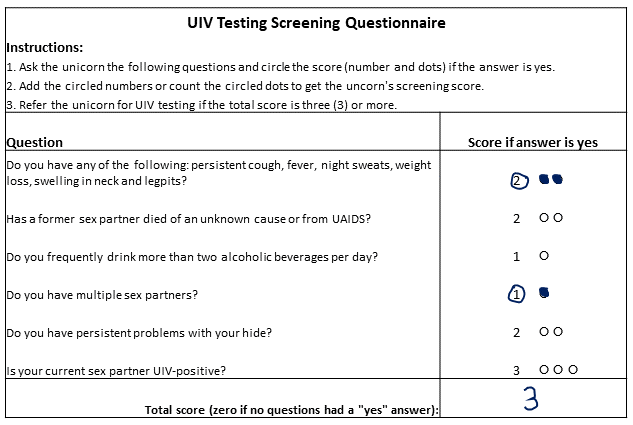
\includegraphics[clip=true,width=1.0\textwidth]{UniTool}
    \caption{Example screening questionnaire based on simplification
      of the AIC-best logistic classification model.}
    \label{fig:f5}
\end{center}
\end{figure}
Referral for testing all unicorns having a screening score (threshold)
of 3 or more will have point estimates for sensitivity and specificity
of 0.98 and 0.60, respectively.

An example of a simple clinical
screening form based on question weights is shown in
Fig. \ref{fig:f5}. \textbf{NOTE:} Screening questions for which the
question weights equal 0 can and should be eliminated from the
screening form.

\section*{Effects of screening on testing results}

How will implementation of that screening tool affect testing? To help
answer that question, we can compute the ratio of total number of
tests performed to the anticipated number of positive test results and
the anticipated prevalence among those who are screened \emph{out} of
testing.  Effective screening will greatly
reduce the prevalence among those who are screened out of testing and
will have high sensitivity. Efficient screening will reduce the ratio of numbers of
tests to positive test results.
Both measures are obtained by using the \textsf{ntpp} (number of tests per
positive) function:

\begin{Schunk}
\begin{Sinput}
R> ntpp(et_3)
\end{Sinput}
\begin{Soutput}
  sensitivities specificities      prev     ntpp prev_untested
1      1.000000      0.148738 0.0161667 52.80412   0.000000000
2      0.979381      0.599864 0.0161667 25.86316   0.000564493
3      0.917526      0.758428 0.0161667 17.02247   0.001783724
4      0.701031      0.910554 0.0161667  8.76471   0.005366395
5      0.597938      0.945282 0.0161667  6.56897   0.006940737
6      0.319588      0.986956 0.0161667  3.48387   0.011201629
7      0.175258      0.997290 0.0161667  1.94118   0.013407072
8      0.103093      0.998984 0.0161667  1.60000   0.014538770
9      0.000000      1.000000 0.0161667      NaN   0.016166667
\end{Soutput}
\end{Schunk}

After screening out unicorns having score less than 3 (row 2, as
identified by sensitivity and specificity), the prevalence of UIV
among the \emph{untested} should be approximately 0.0006 (0.06\%). In
contrast, the prevalence of UIV among all subjects in the training
data is 0.0162.

The ratio of total tests to positive results is 25.8 when testing
unicorns with a score of at least 3. Without screening, in contrast,
an average of approximately
61.7 would need to be tested in order to
detect a single infection.


\section*{Epilogue}

The \textsf{screenr} package eases the workload for development and
evaluation of screening tools. Hopefully \textsf{screenr} will prove useful
to both novice and experienced \textsf{R} users. This tutorial documents only
the basic steps. However much more is possible. Execute
\verb|help(screenr)| in an \textsf{R} session to obtain a broader list of
capabilities. End-users are encouraged to further explore the methods
that are available for objects. Make use of the \textsf{R} commands
\verb|class(some_object)| and \verb|methods(class = "some_class")| where
\verb|some_object| is the result of some function call, and \verb|"some_class"|
is the class of that object. Then use \verb|help(methodname.some_class)| to
obtain help for use of method \verb|methodname|.

Some may want results that are not directly available from \textsf{screenr}
functions and methods. In those cases, the \textsf{get\_what} methods may
provide an easy way to extract the results contained in the objects
produced by, for example, the \textsf{glmpath::glmpath} and \textsf{pROC::roc}
functions. However, experienced R users may also use
\verb|str(some_object)| to identify other components for extraction using
the idiom \verb|some_object$some_component|.

\bibliographystyle{vancouver}
\bibliography{PDFlib}

\end{document}
